\documentclass{article}
\usepackage[utf8]{inputenc}
\usepackage{amsmath}
\usepackage{indentfirst}
\usepackage{graphicx,caption}
\usepackage[a4paper, margin=1in]{geometry}
\linespread{1.15}
\usepackage{empheq}
\usepackage[most]{tcolorbox}
\usepackage[margin=3cm]{caption}

\usepackage{xcolor,sectsty}
\definecolor{astral}{RGB}{46,116,181}
\subsectionfont{\color{astral}}
\sectionfont{\color{astral}}

\title{
\includegraphics[width=0.1\textwidth]{ufallogo.png} \\\Huge{\color{astral}\textbf{Mecânica Não-Linear e Caos}}}
\author{Paulo Brandão}
\date{Maio de 2017}

\newtcbox{\mymath}[1][]{%
    nobeforeafter, math upper, tcbox raise base,
    enhanced, colframe=blue!30!black,
    colback=blue!30, boxrule=1pt,
    #1}

\begin{document}

\maketitle

\section{Introdução}

A segunda lei de Newton nos permite calcular a trajetória $\mathbf{r}(t) = [x(t),y(t),z(t)]$ de uma partícula com massa $m$ que está sob ação de um conjunto de forças cuja resultante é $\mathbf{F}$ através da relação $m\ddot{\mathbf{r}} = \mathbf{F}$, onde o ponto duplo $\ddot{ }$ acima da variável indica uma derivada de segunda ordem no tempo. Iremos assumir que a força resultante $\mathbf{F}$ pode depender apenas da posição $\mathbf{r}$, da velocidade $\mathbf{\dot{r}}$ e, de forma explícita, do tempo $t$ \footnote{A construção de uma teoria da mecânica clássica coerente onde a força depende da aceleração da partícula, ainda está em debate! Para o aluno mais interessado nesses assuntos, veja, por exemplo, a referência \textit{J. Appl. Mech 79 (4), 04450 (2012)}}. A estratégia a ser seguida após identificar a força resultante é: resolver a equação diferencial para obter a posição do corpo em função do tempo, isto é, sua trajetória $\mathbf{r}(t)$. A grande dificuldade com esse método é que a força resultante pode se tornar bastante complicada, dependendo da sua relação com as variáveis $\mathbf{r}$, $\mathbf{\dot{r}}$ e $t$. Em geral, dividimos a equação diferencial $m\ddot{\mathbf{r}} = \mathbf{F}$ em duas classes: equações diferenciais lineares e não-lineares. A diferença entre essas duas classes será discutida na seção 2. Após identificar a força resultante $\mathbf{F}$ e substituí-la na equação diferencial, podemos concluir (erroneamente) que o sistema é completamente determinístico. Isto é, dadas as condições iniciais $(\mathbf{r}_0,\mathbf{\dot{r}}_0)$, a trajetória da partícula é obtida para qualquer valor de tempo $t$ e para quaisquer condições iniciais (e para qualquer força resultante). Uma das descobertas mais fascinantes das últimas décadas foi o reconhecimento de que a maioria dos sistemas regidos por equações não-lineares pode exibir \textbf{caos}. Esse fenômeno não-trivial quer dizer que, apesar do sistema satisfazer equações determinísticas do movimento, o seu comportamento futuro pode, de uma maneira prática, não ser previsível. A seção 3 descreve um modelo mecânico não-linear muito simples mas que nos possibilita estudar o aparecimento de um comportamento caótico dependendo de certos parâmetros presentes no sistema. A seção 4 apresenta um fenômeno muito importante chamado de duplicamento de período que aparece um pouco antes do sistema atingir o comportamento caótico. Na seção 5 iremos quantificar o caos no pêndulo forçado amortecido e estudar sua sensibilidade às condições iniciais bem como introduziremos algumas quantidades importantes como o Expoente de Liapunov. Finalizaremos na seção 6 com os diagramas de Bifurcação, que são construções úteis para caracterizar o caos no sistema.

\section{Força Linear e Não-Linear}

Apesar da enorme quantidade de equações diferenciais existentes, podemos classificá-las em dois conjuntos: lineares e não-lineares. Vamos assumir daqui em diante que o sistema seja descrito de forma completa por apenas uma variável a qual chamaremos de $x(t)$. A variável $x$ não precisa ser necessariamente uma posição espacial no eixo $x$. Ela pode representar, por exemplo, o ângulo $\phi$ entre a vertical e o fio de um pêndulo. Em uma dimensão, a força $F_x$ (que chamaremos simplesmente de $F$), depende portanto das variáveis $x$, $\dot{x}$ e, possivelmente, do tempo $t$ de forma explícita. Uma equação diferencial é linear se ela envolve a variável dependente $x$ e a sua derivada $\dot{x}$ linearmente. A forma mais geral, em uma dimensão, pode ser escrita como \footnote{Quando uma equação diferencial envolve apenas derivadas ordinárias, isto é, não envolve derivadas parciais, chamamos de \textit{ordinária}.}
\begin{equation}
    F(x,\dot{x},t) = ax + b\dot{x} + g(t),
    \label{linear}
\end{equation}
onde $a$ e $b$ são números reais e $g(t)$ uma função real que depende somente do tempo $t$. A segunda lei de Newton na forma linear é dada por
\begin{equation}
    m\ddot{x} = ax + b\dot{x} + g(t).
    \label{edol}
\end{equation}
Se o termo $g(t)$ for nulo, dizemos que a equação é homogênea. Caso contrário, ela será não-homogênea. Exemplos de sistemas lineares homogêneos ($g =0$) foram estudados no início do curso. O oscilador massa-mola simples é descrito por $m\ddot{x} = -kx$, onde $k$ é a constante da mola, que é um caso especial da relação \eqref{edol} com $a = -k$ e $b = 0$. O oscilador massa-mola amortecido é descrito pela equação $m\ddot{x} = -kx-\gamma\dot{x}$, onde $\gamma$ é a constante de amortecimento, que é um caso especial da relação \eqref{edol} com $a=-k$ e $b = -\gamma$. Caso o oscilador massa-mola simples amortecido esteja sob ação de uma força externa variável $F(t)$, seu movimento é regido pela equação $m\ddot{x} = -kx-\gamma\dot{x} + F(t)$ que é um caso especial da relação \eqref{edol} com $a = -k$, $b = -\gamma$ e $g(t) = F(t)$. A grande vantagem, em termos práticos, de descrever um sistema regido por uma equação linear é que, geralmente, ele é muito simples de ser resolvido. Existem métodos matemáticos eficientes para resolver equações do tipo \eqref{edol}. Além disso, equações diferenciais lineares satisfazem o poderoso \textit{princípio da superposição}: Se $x_1(t)$ e $x_2(t)$ são soluções de uma equação diferencial linear da forma $\eqref{edol}$, então $x(t) = c_1 x_1(t) + c_2 x_2(t)$ também é solução, onde $c_1$ e $c_2$ são constantes arbitrárias. O estudante demonstrará esse fato na lista de exercícios.

Por outro lado, a grande classe de problemas mecânicos práticos envolvem equações diferenciais não-lineares. Nesse caso, a força não é escrita em termos lineares de $x$ e $\dot{x}$. Exemplo de sistemas que são descritos por equações diferenciais ordinárias não-lineares (EDONL), apesar de muito abundantes, não são descritos de forma aprofundada em livros-texto. O motivo é simples: EDONL, em geral, são muito complicadas de se resolver analiticamente. Existe um número muito pequeno de problemas não-lineares (isto é, problemas que são descritos por uma EDONL) onde a solução analítica é conhecida. O movimento de um único planeta de massa $m$ no campo do sol de massa $M$, por exemplo, descrito por
\begin{equation}
    m\mathbf{\ddot{r}} = -G\frac{mM\mathbf{\hat{r}}}{r^2},
\end{equation}
onde  $G$ é a constante gravitacional, foi solucionado por Newton e sabemos que o resultado analítico é dado em termos de uma trajetória elíptica. Um outro sistema não-linear que possui solução analítica é o movimento de uma partícula num fluido viscoso que produz uma força de amortecimento do tipo $-bv^2 = -b\dot{x}^2$, descrito por $m\ddot{x} = -b\dot{x}^2$, onde o termo não-linear é $\dot{x}^2$. Um último exemplo de sistema não-linear mas que possui uma solução analítica é o pêndulo descrito por $m\ddot{x} = -mgL\sin x$, onde $L$ representa o comprimento do fio e $x$ o ângulo entre a vertical e o fio. Apesar da existência do termo não-linear ($\sin x$), é possível obter uma solução analítica para o problema. Note que esses três exemplos não são casos especiais da relação \eqref{edol}. Infelizmente, a grande maioria dos sistemas não-lineares são tão complicados que é \textbf{impossível} obter uma solução analítica. De fato, os casos mais especiais são os problemas lineares! A grande maioria dos sistemas possui uma equação de movimento não-linear.

Não-linearidade é essencial para se obter caos num sistema. Se as equações de movimento do sistema foram lineares, ele não pode exibir um comportamento caótico. Mas a não-linearidade não garante o surgimento do caos. Por exemplo, a equação $m\ddot{x} = -mgL\sin x$ para o pêndulo é não-linear, mas mesmo quando a amplitude do movimento é grande (onde a aproximação linear não é boa) o pêndulo nunca exibe caos.

\section{Modelo Proposto Para Estudar Caos}

É possível estudar as características de um movimento caótico através da análise geral de equações diferenciais não-lineares, sem escolher um modelo específico. Esse tipo de didática é útil em um nível mais avançado onde o aluno (ou o pesquisador) já possui uma certa noção sobre o tema. Entretanto, como estamos num nível de graduação, escolhemos caminhar por outra rota. Nossa análise consistirá na escolha de um modelo físico simples (que pode executar um movimento caótico) e aos poucos iremos observar o que acontece com o sistema na medida em que ele se aproxima de um movimento considerado caótico.  

Dentre todos os modelos físicos possíveis que exibem caos, vamos escolher o pêndulo forçado amortecido (PFA), como indica a Figura 1. Para derivar a equação do movimento, vamos utilizar a relação entre torque e momento angular:
\begin{equation}
    \frac{d\mathbf{L}}{dt} = \frac{d}{dt}\mathbf{r}\times\mathbf{p} = \mathbf{r}\times\mathbf{F}_R = \mathbf{N},
    \label{eq4}
\end{equation}
onde $\mathbf{L}$ é o momento angular e $\mathbf{F}_R$ a força resultante na partícula. Se escolhermos o eixo $y$ no sentido da força peso $\mathbf{P}$, então a posição da partícula é dada por $\mathbf{r} = L\sin\phi\hat{x} + L\cos\phi\hat{y}$ e a velocidade vale $\mathbf{v} = \dot{\mathbf{r}} = L\dot{\phi}\cos\phi\hat{x} - L\dot{\phi}\sin\phi\hat{y}$. O momento angular é facilmente obtido:
\begin{equation}
    \mathbf{L} = \mathbf{r}\times m\mathbf{\dot{r}} = -mL^{2}\dot{\phi}\hat{z}.
    \label{eq5}
\end{equation}
O torque $\mathbf{N}$ é composto por três partes, uma para cada força que atua no objeto. Temos a força peso $\mathbf{P}$, a força resistiva $\mathbf{F}_\text{at}$ e a força externa $\mathbf{F}_\text{ext}$. Assim,
\begin{equation}
    \mathbf{N} = \mathbf{r}\times\mathbf{P} +\mathbf{r}\times\mathbf{F}_\text{at} + \mathbf{r}\times\mathbf{F}_{ext} = mgL\sin\phi\hat{z} + bL^{2}\dot{\phi}\hat{z} - LF(t)\hat{z},
    \label{eq6}
\end{equation}
e, após substituir as equações \eqref{eq5} e \eqref{eq6} na equação \eqref{eq4}, obtemos a equação do movimento:
\begin{equation}
    \ddot{\phi} + \frac{b}{m}\dot{\phi} + \frac{g}{L}\sin\phi = \frac{F_0}{mL}\cos\omega t,
\end{equation}
onde $b$ é a constante de amortecimento, $L$ o comprimento do fio e escolhemos a força externa como periódica com amplitude $F_0$ e frequência angular $\omega$. Para colocar o problema numa forma mais fácil de identificar certos parâmetros importantes, vamos definir as seguintes quantidades:
\begin{itemize}
    \item $b/m = 2\beta$,
    \item $g/L = \omega_0^2$,
    \item $\gamma = F_0/mL\omega_0^2 = F_0/mg$.
\end{itemize}
Da lista acima, o parâmetro mais importante para nós será $\gamma$. Ele é dado pela razão entre a amplitude da força externa $F_0$ e a força peso $mg$ que atua na partícula. Quanto maior for $\gamma$, mais a partícula responderá com relação à força externa e vice-versa. A Figura 1 ilustra o sistema físico junto com as forças que atuam na partícula.
\begin{figure}[h]
\centering
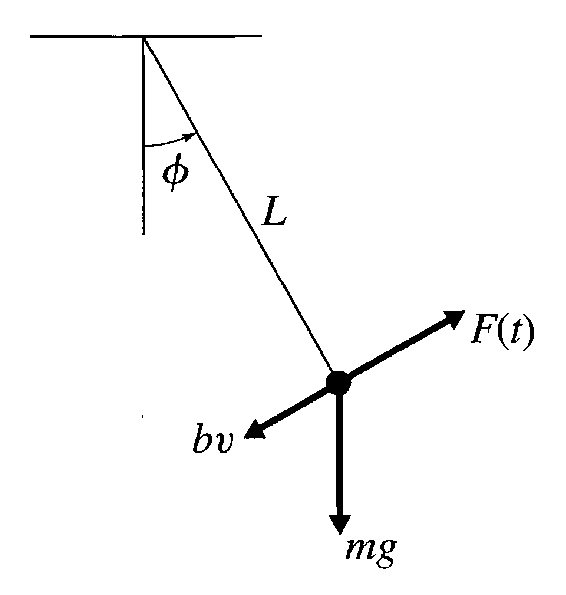
\includegraphics[width=4cm]{forcedpen.png}
\captionsetup{labelsep=none}
\caption{. Pêndulo forçado com perda. A força $F(t)$ atua na direção tangente à trajetória do pêndulo.}
\end{figure}
Após fazer as substituições acima, a equação geral do movimento do PFA pode ser escrita como
\begin{empheq}[box=\tcbhighmath]{equation*}
    \ddot{\phi} + 2\beta\dot{\phi} + \omega_0^2\sin\phi = \gamma\omega_0^2\cos\omega t.
\end{empheq}
Essa é a equação cujas soluções estaremos estudando nas próximas seções.

\section{A Rota Para o Caos}

O comportamento da massa no pêndulo depende, de uma forma geral, das condições iniciais e do valor de $\gamma$. Vamos supor que a frequência $\omega$ da força externa seja $\omega = 2\pi$ de tal forma que seu período seja $\tau = 2\pi/\omega = 1$ e que o sistema esteja fora da ressonância, $\omega_0 = 1.5\omega$. Vamos considerar também que a constante de amortecimento seja $\beta = \omega_0/4$ e que as condições iniciais satisfaçam $\phi(0) = -\pi/2$ e $\dot{\phi}(0) = 0$ (ou seja, a massa é solta inicialmente com velocidade nula na posição $x = -L$ e $y = 0$ [veja a figura 1]). O próximo passo é variar os valores de $\gamma$ e observar o movimento resultante.

\subsection{Duplicação de Período}

Quando o parâmetro $\gamma$ é muito menor que 1, esperamos que o sistema se comporte mais ou menos como no caso linear. Nesse regime, o movimento da massa deve ser dado, pelo menos após os transientes, aproximadamente por uma função periódica com período igual ao da força externa, no caso $\tau = 1$. Entretanto, à medida que aumentamos o valor de $\gamma$, encontramos um valor bem específico $\gamma_1$ onde o sistema é caracterizado por uma dinâmica diferente. Para os valores escolhidos de $\beta$, $\omega_0$, etc, acima, temos que quando $\gamma_1=1,0663$ o movimento periódico (após os transientes) possui o período duas vezes maior que o período $\tau = 1$. Em outras palavras, a partícula, após um longo tempo, executa um movimento periódico com período igual à duas vezes o período da força externa. Se aumentarmos ainda mais o valor de $\gamma$ de tal forma que ele ultrapasse o segundo valor $\gamma_2 = 1,0793$, o movimento da massa (após os transientes) é periódico com período 4, isto é, duas vezes o período anterior quando $\gamma < \gamma_1$. O caso geral é ilustrado pela Tabela 1. 

\begin{figure}[h]
\centering
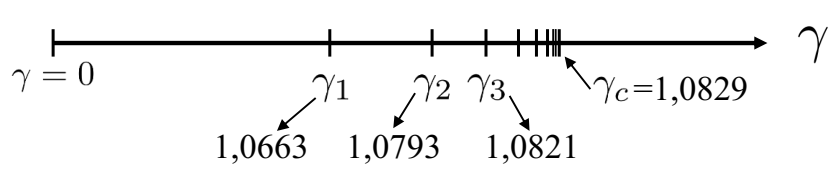
\includegraphics[width=8cm]{fig2.png}
\captionsetup{labelsep=none}
\caption{. A figura mostra os pontos principais de $\gamma$, num eixo linear, onde ocorre a duplicação de período do movimento do pêndulo até atingir um valor crítico $\gamma_c$. }
\end{figure}
 
\begin{table}[h!]
\centering
\begin{tabular}{||c c||} 
 \hline
 Intervalo em $\gamma$ & Período (após os transientes) \\ [0.5ex] 
 \hline\hline
 $0 < \gamma < \gamma_1$ & 1 \\ 
 $\gamma_1 < \gamma < \gamma_2$ & 2 \\
 $\gamma_2 < \gamma < \gamma_3$ & 4 \\
 $\gamma_3 < \gamma < \gamma_4$ & 8 \\
 $\gamma_4 < \gamma < \gamma_5$ & 16 \\ [1ex] 
 \hline
\end{tabular}
\caption{Essa tabela ilustra os intervalos dos valores de $\gamma$ e seus respectivos períodos após os transientes.}
\label{table:1}
\end{table}

É facil perceber que as distâncias entre $\gamma_n$ e $\gamma_{n+1}$ diminuem à medida que $n$ aumenta. No final dos anos 70, o físico Mitchell Feigenbaum não apenas mostrou que muitos sistemas não-lineares possuiam esse fenômeno de duplicação de período, mas descobriu também que os intervalos entre $\gamma_n$ e $\gamma_{n+1}$ diminuiam por uma razão geométrica. Em termos quantitativos, o número $\delta$ dado por
\begin{equation}
    \delta = \frac{\gamma_n - \gamma_{n-1}}{\gamma_{n+1} - \gamma_n},
\end{equation}
é uma constante, chamada \textit{número de Feigenbaum}. A relação acima é válida apenas quando $n\rightarrow\infty$, porém alguns sistemas podem possuir uma razão entre os intervalos muito próxima ao número de Feigenbaum quando $n$ é pequeno. O valor de $\delta$ é 
\begin{empheq}[box=\tcbhighmath]{equation*}
    \text{\textbf{Número de Feigenbaum}: }\delta = 4,6692016.
\end{empheq}
Dessa forma, cada intervalo sucessor é menor que o anterior por um fator de $1/\delta \approx 0,21$. A relação de Feigenbaum implica que os intervalos entre os limites sucessivos de $\gamma_n$ aproximam-se de zero rapidamente, e portanto que os próprios limites $\gamma_n$ se aproximam de um limite finito $\gamma_c$
\begin{equation}
    \gamma_n \rightarrow \gamma_c \hspace{1cm}(\text{quando } n\rightarrow \infty).
\end{equation}
Portanto, a sequência dos valores limites satisfazem a desigualdade
\begin{equation}
    \gamma_1 < \gamma_2 < ... < \gamma_n < ... < \gamma_c
\end{equation}
com valores infinitos de $\gamma_n$ espremidos no curto intervalo entre $\gamma_n$ e $\gamma_c$. Para o sistema que estamos considerando (PFA), o limite $\gamma_c$ é calculado como sendo
\begin{equation}
    \gamma_c = 1,0829.
\end{equation}
Nós iremos ver que além do valor crítico $\gamma_c$, surge o caos, e, portanto, o fenômeno de duplicação do período é chamado de uma \textbf{rota para o caos}. Entretanto, devemos enfatizar que nem todos os sistemas apresentam caos sem primeiro passar pelo fenômeno de duplicação de período. Isto é, a duplicação do período é apenas uma de várias rotas que levam ao caos.



\section{Caos e Condições Iniciais}

Se aumentarmos o valor de $\gamma$ para além do valor crítico $\gamma_c = 1,0829$, o PFA começa a exibir o comportamento que chamaremos de ``caótico''. A Figura 3 ilustra o gráfico da ``posição''$\phi(t)$ no decorrer do tempo para $\gamma = 1,105$, $\phi(0) =\pi/2$, $\dot{\phi}(0) = 0$ e os outros parâmetros são os mesmos considerados anteriormente. O movimento é errático e nunca se repete em qualquer intervalo temporal considerado. Um gráfico de qualquer intervalo temporal é tão errático quanto qualquer outro intervalo. Em outras palavras, no longo tempo, o movimento não se torna periódico. Esse movimento não-periódico e errático é uma das características de um movimento caótico. A outra característica é a sensibilidade às condições iniciais.


\begin{figure}[h]
\centering
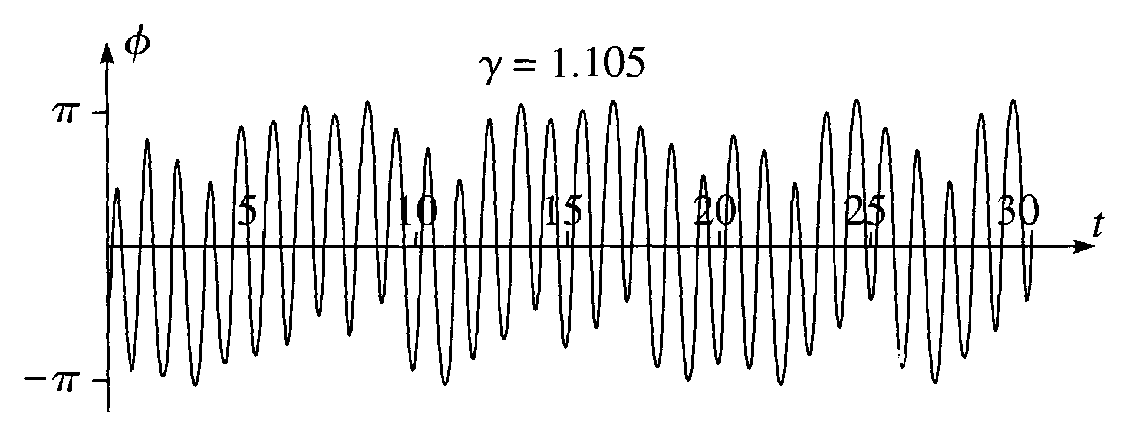
\includegraphics[width=8cm]{pend1.png}
\captionsetup{labelsep=none}
\caption{. Movimento caótico. Os primeiros 30 ciclos do PFA com $\gamma = 1,105$ são erráticos e não mostram sinais de periodicidade. De fato, as oscilações nunca se transformam em um movimento regular periódico. Esse movimento erratico, não-periódico, de longo alcance, é uma das características do movimento caótico. }
\end{figure}

\subsection{Sensibilidade às Condições Iniciais}

Dados dois PFA idênticos, o que acontece com o movimento das duas massas, $\phi_1(t)$ e $\phi_2(t)$, no decorrer do tempo, caso as condições iniciais sejam ligeiramente diferentes? Por exemplo, se $\phi_1 (0) = \pi/2$ e $\phi_2 (0) = \phi_1 (0)/1000$ (ambas porém com velocidade inicial nula), como será a evolução da \textit{diferença} entre as duas soluções: $\Delta \phi(t) = \phi_2 (t) - \phi_1 (t)$? Para o oscilador \textit{linear} a resposta é que $\Delta\phi(t)$ vai para zero \textbf{exponencialmente}. Para compreender esse fato, lembre-se de que a equação do oscilador linear é dada por
\begin{equation}
    \ddot{\phi} + 2\beta\dot{\phi} + \omega_{0}^{2}\phi = \gamma\omega_{0}^{2}\cos\omega t,
\end{equation}
cuja solução geral pode ser escrita na forma
\begin{equation}
    \phi(t) = A\cos(\omega t - \theta) + C_1 e^{r_1 t} + C_2 e^{r_2 t}.
\end{equation}
O termo de cosseno é o mesmo para todas as soluções, enquanto que os dois termos exponenciais possuem coeficientes $C_1$ e $C_2$ que dependem das condições iniciais. Assim, para duas soluções com apenas as condições iniciais diferentes, temos
\begin{equation}
    \Delta\phi(t) = B_1 e^{r_1 t} + B_2 e^{r_2 t}.
\end{equation}
Os parâmetros $r_1$ e $r_2$ são, em geral, números complexos da forma $-\beta \pm i\omega_1$, de modo que podemos escrever a equação para $\Delta\phi(t)$ como
\begin{equation}
    \Delta\phi(t) = D e^{-\beta t}\cos(\omega_1 t - \theta).
\end{equation}
É útil utilizar no lugar da função $\Delta\phi(t)$, o logaritmo do seu módulo. Dessa forma, temos que
\begin{equation}
    \ln{|\Delta\phi(t)|} = \ln D - \beta t + \ln{|\cos(\omega_1 t - \theta)|},
\end{equation}
onde fica fácil de perceber que um gráfico de $\ln{|\Delta\phi(t)|}$ mostrará uma variação periódica (último termo da relação acima) superposta numa reta (segundo termo da relação acima). A Figura 4 mostra a solução numérica da equação do movimento considerando $\gamma = 0.1$, que é um valor menor que $\gamma_1$ e, portanto, o pêndulo deve oscilar com a frequência da força $F(t)$. É fácil de ver as características do decaimento linear superpostos na variação periódica. Os picos para baixo aparecem quando o termo envolvendo cosseno vale zero, de forma que o logaritmo vai para (menos) infinito.

\begin{figure}[h]
\centering
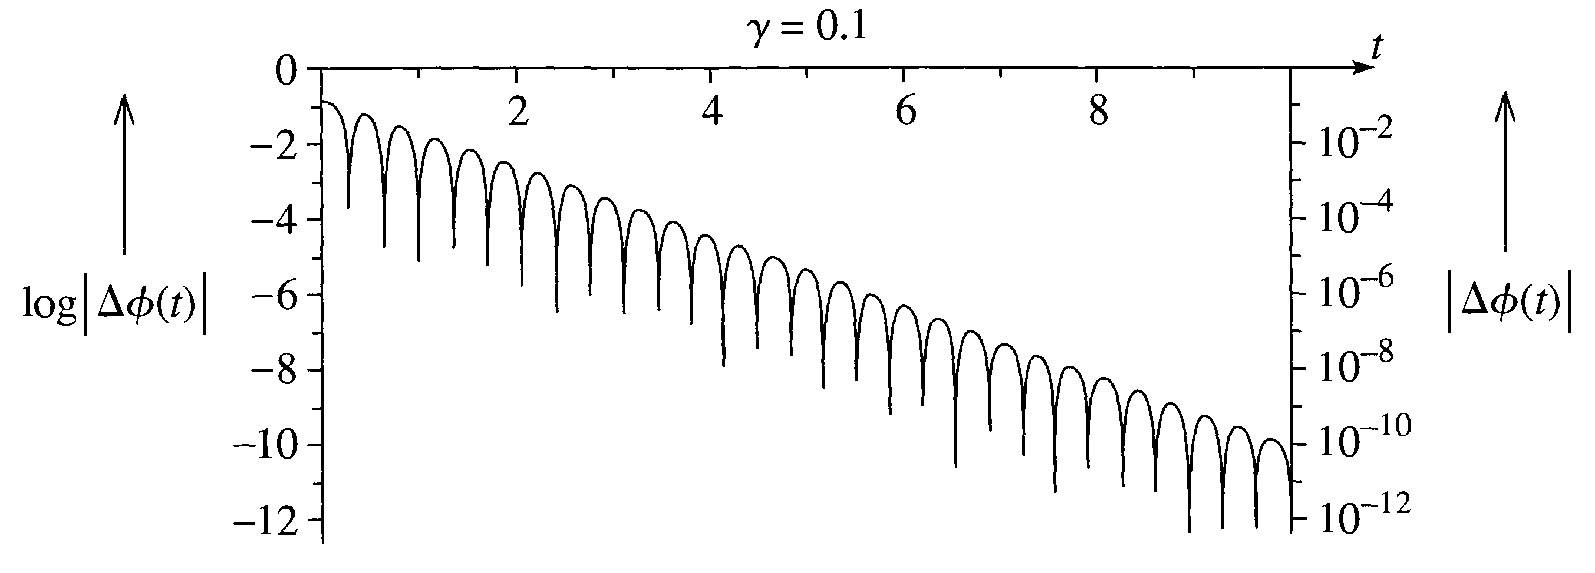
\includegraphics[width=8cm]{pend2.png}
\captionsetup{labelsep=none}
\caption{. Gráfico de $\log{|\Delta\phi(t)|}$ quando $\gamma = 0.1$ (regime linear). A diferença inicial entre os dois ângulos foi de 0.1 radianos (aproximadamente 6$^o$). }
\end{figure}

O comportamento da variação linear do gráfico (e consequentemente, da variação exponencial negativa das duas soluções) acontece para todos os valores de $\gamma$ menores que $\gamma_c$. Se agora aumentarmos o valor de $\gamma$ para além de $\gamma_c$, dentro do regime caótico, esse comportamento muda completamente. A figura 5 mostra a evolução de $\ln{|\Delta\phi (t)|}$ para $\gamma = 1,105$ (acima de $\gamma_c$) quando os ângulos iniciais diferem de $10^{-4}$ radianos. Observamos que o gráfico \textit{cresce linearmente} com o tempo, o que implica que a diferença entre os dois ângulos cresce \textbf{exponencialmente}. O crescimento exponencial implica que uma pequena diferença entre os dois ângulos iniciais rapidamente cresce em uma grande incerteza na predição do movimento. É nesse sentido que dizemos que o caos possui \textbf{uma sensibilidade extrema às condições iniciais} e é essa sensibilidade que faz com que a predição confiável da evolução do sistema se torne uma impossibilidade prática.

\begin{figure}[h]
\centering
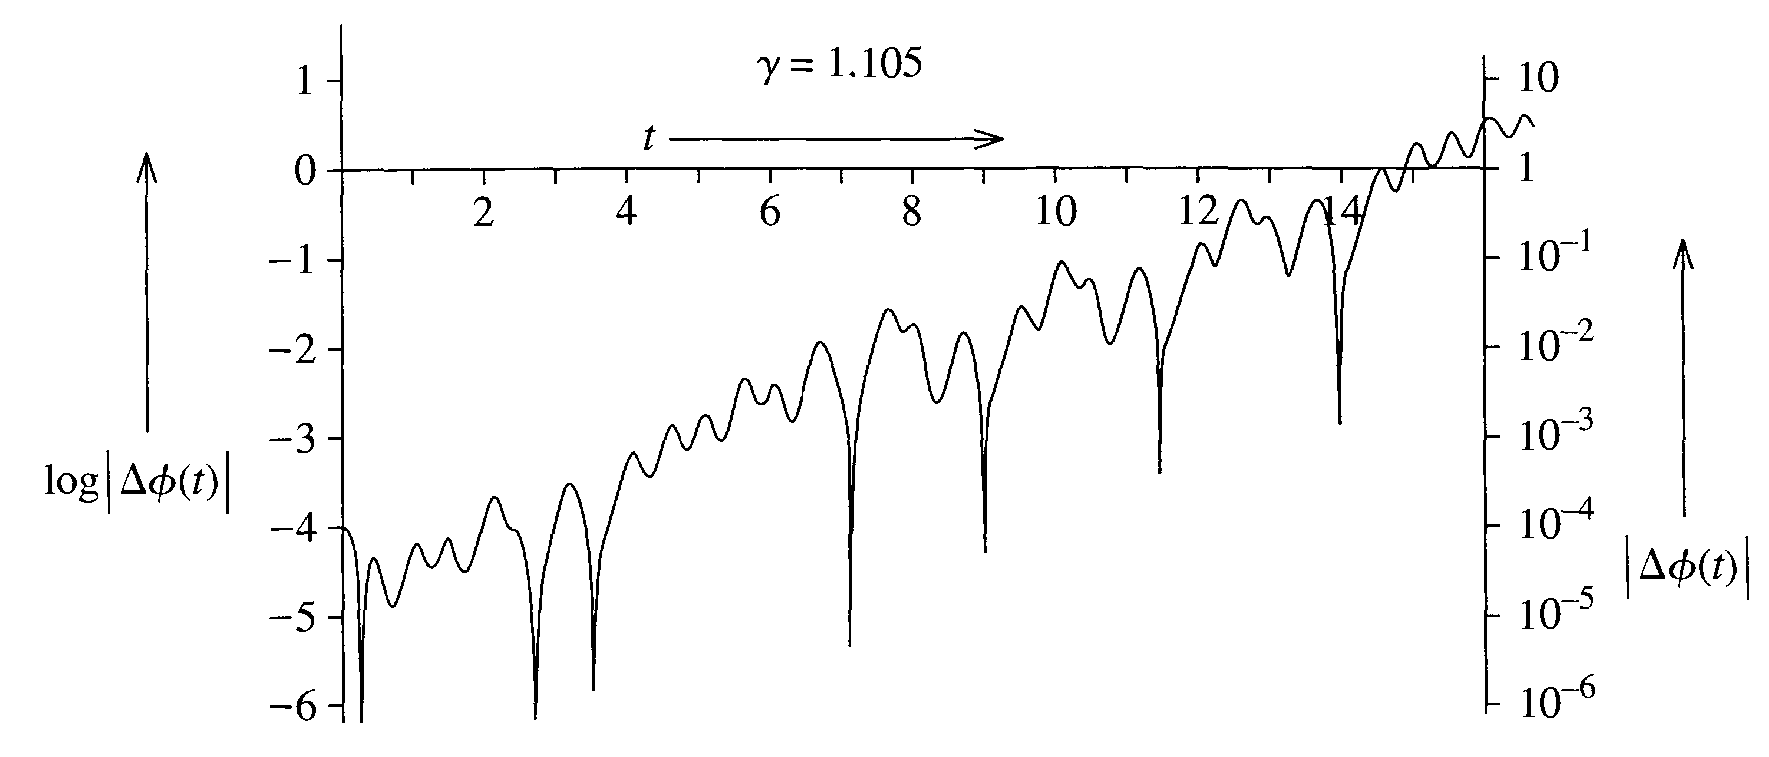
\includegraphics[width=8cm]{pend3.png}
\captionsetup{labelsep=none}
\caption{. Gráfico de $\log{|\Delta\phi(t)|}$ quando $\gamma = 1,105$ (regime caótico). A diferença inicial entre os dois ângulos foi de $10^{-4}$ radianos. }
\end{figure}

\subsection{O Expoente de Lyapunov}

A análise anterior sugere que a diferença $\Delta\phi(t)$ entre dois PFA idênticos soltos com condições iniciais ligeiramente diferentes se comporta de forma exponencial:

\begin{equation}
    |\Delta\phi(t)| \sim Ke^{\lambda t},
\end{equation}
onde o símbolo $\sim$ significa que $\Delta\phi(t)$ pode oscilar por baixo de um envelope com o comportamento exponencial e $K$ é uma constante. O coeficiente $\lambda$ é chamado \textbf{expoente de Liapunov}. Se, após um grande período de tempo, o movimento se tornar periódico, o coeficiente de Liapunov é negativo; se o movimento se tornar errático e não-periódico, o coeficiente de Liapunov é positivo.


\subsection{O Caso $\gamma > \gamma_c$}

Você pode pensar que aumentando o valor de $\gamma$ além de $\gamma_c$ apenas aumentaria a intensidade do movimento caótico do sistema. No entanto, sistemas não-lineares não podem ser pensados de forma ``intuitiva" com o mesmo conhecimento que possuímos de sistemas lineares. De fato, aumentando o valor de $\gamma$ faz com que o sistema alterne entre intervalos caóticos e intervalos onde o movimento é periódico não-caótico. 



\section{Diagramas de Bifurcação}

Em todos os gráficos feitos até agora, sempre plotamos o ângulo $\phi$ em fução do tempo $t$. Com isso obtemos uma relação direta entre o comportamento da massa do pêndulo no decorrer do tempo para um determinado valor de $\gamma$. Infelizmente, observar um movimento caótico olhando apenas para gráficos desse tipo é bastante complicado. Precisamos de uma maneira de reunir todas as informações do movimento em um único gráfico para todos os valores possíveis de $\gamma$. Essa é a ideia por trás dos diagramas de bifurcação, como iremos discutir agora.

Vimos que quando $\gamma < \gamma_1$, o pêndulo apresenta (para $t$ grande) um movimento periódico com período igual ao período da força externa $F(t)$ que assumimos ser $\tau = 1$. Suponha que calculamos os valores de $\phi(t)$ para valores de $t$ espaçados pelo período, por exemplo, $\phi(500)$, $\phi(501)$, $\phi(502)$, $\phi(503)$, e assim por diante. Fica claro que todos esses valores serão iguais (ou extremamente próximos), já que o sistema oscila periodicamente com período igual ao intervalo $\Delta t$ escolhido. Se fizermos a mesma análise para valores do parâmetro $\gamma$ no intervalo $\gamma_1<\gamma<\gamma_2$, sabemos que o sistema está com o período duplicado, e se, mais uma vez, verificarmos os valores $\phi(500)$, $\phi(501)$, $\phi(502)$, $\phi(503)$, etc, obteríamos dois números diferentes. Um diagrama de bifurcação é construído escolhendo dois eixos onde um deles representa os valores de $\gamma$ e o outro os valores que não são repetidos de $\phi(500)$, $\phi(501)$, $\phi(502)$, $\phi(503)$, etc. 

\begin{figure}[h]
\centering
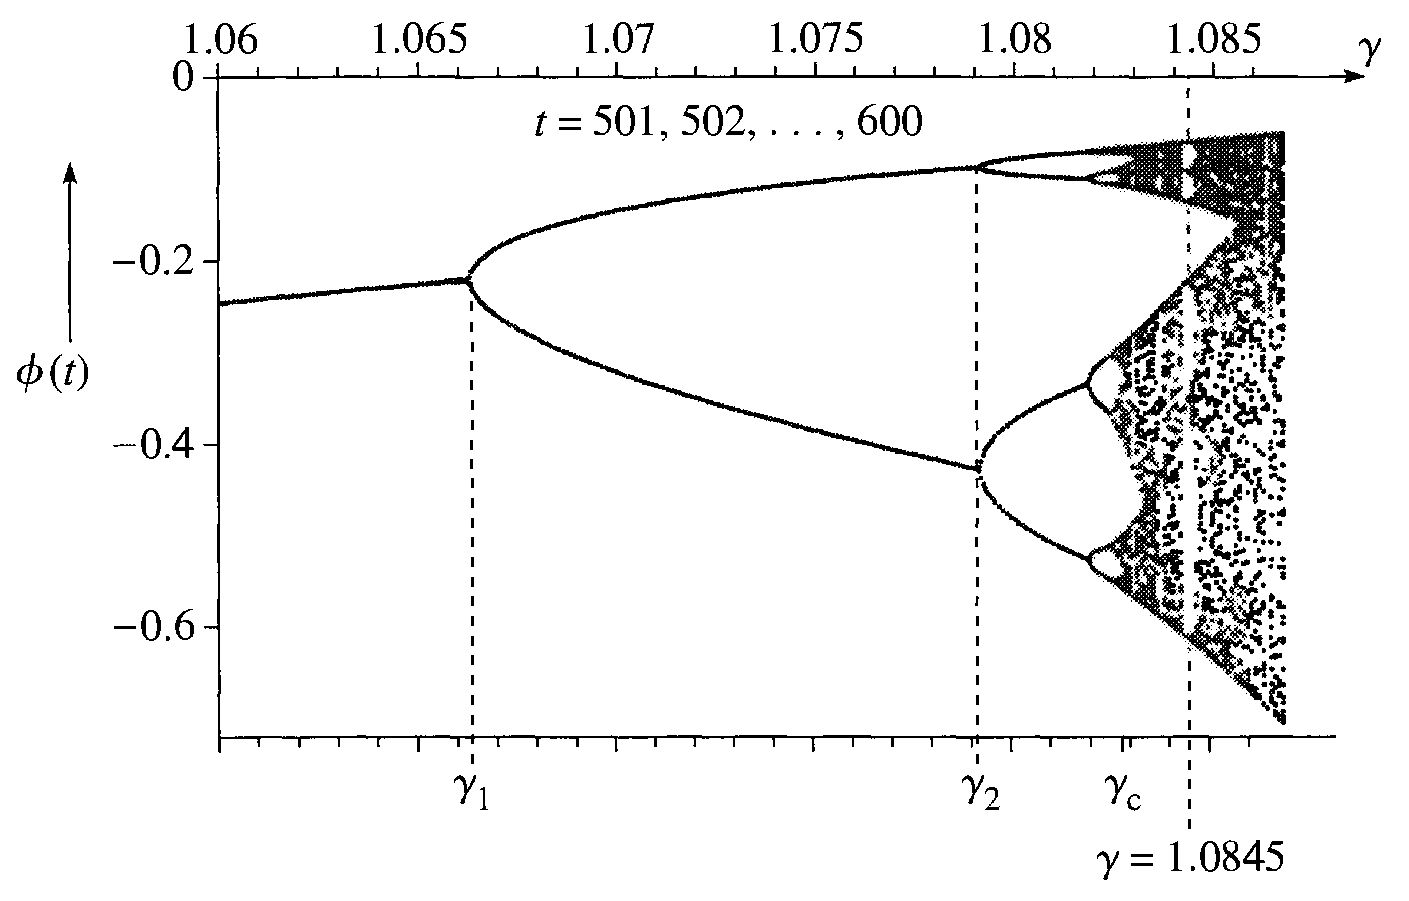
\includegraphics[width=8cm]{bif.png}
\captionsetup{labelsep=none}
\caption{. Gráfico de $\log{|\Delta\phi(t)|}$ quando $\gamma = 1,105$ (regime caótico). A diferença inicial entre os dois ângulos foi de $10^{-4}$ radianos. }
\end{figure}

A Figura 6 ilustra o diagrama de bifurcação para o PFA considerado nesta aula. Observe que para $\gamma < \gamma_1$ apenas um ``ponto'' aparece pra cada valor de $\gamma$ nesse intervalo, indicando que o movimento possui o período igual ao período da força $F(t)$, isto é, 1. Para $\gamma$ no intervalo $\gamma_1 < \gamma < \gamma_2$ obervamos dois pontos para cada valor de $\gamma$ nesse intervalo, o que indica um período igual a dois. É possível observar na Figura 6 o comportamento do pêndulo para o período igual a 4 e 6. Quando $\gamma > \gamma_c$, o gráfico se torna uma confusão sólida de pontos e é impossível dizer (olhando o gráfico, pelo menos) o valor exato de $\gamma_c$ onde o caos começa. Além desse ponto, o gráfico é praticamente caótico com uma pequena janela indicada pela linha tracejada na figura onde ocorre a presença de 6 pontos distintos, indicando que, para esse valor específico de $\gamma$ (aproximadamente 1,0845), o movimento possui um período igual a 6. 

\section{O que vem depois?}

Claramente, o estudo de sistemas caóticos é muito complexo de forma que é impossível falar de todos os seus aspectos numa única aula. Nada foi dito sobre os atratores do sistema, apesar de que sua introdução poderia ser feita de forma muito fácil em termos gerais das equações diferenciais. O próximo passo lógico seria introduzir as órbitas no espaço-estado (ou trajetórias no espaço de fase), que formam uma nova maneira de olhar para o movimento do sistema. O curso continuaria com a discussão das seções de Poincaré e, finalmente, sobre os mapas logísticos. Iremos abordar esses assuntos em um outro momento mais oportuno.

\end{document}
